\documentclass[../main.tex]{subfiles}
\graphicspath{{\subfix{../images/}}, {\subfix{../}}}

\begin{document}

\chapter{Introduction}\label{ch:introduction}

The United Nations declared 2025 the `International Year of Quantum Science and Technology' \cite{unitednationsInternationalYearQuantum2024}.
This is an effort to raise awareness of the importance of quantum science and its applications, focusing on 3 key areas: quantum computing, quantum communications and quantum sensors.

One effect underlying many of these applications is the phenomenon of superconductivity, a phase of matter characterized by vanishing electrical resistance and expulsion of magnetic fields.
For example, superconducting qubits are a promising platform for scalable quantum computing \cite{huangSuperconductingQuantumComputing2020, aruteQuantumSupremacyUsing2019} and the Josephson effect \cite{josephsonPossibleNewEffects1962} can be used to build extremely sensitive measurement devices for magnetic fields \cite{faleyHighTcSQUIDBiomagnetometers2017} or voltages \cite{klushinPresentFutureHightemperature2020}.

\subsection*{Superconductivity}

Superconductivity was discovered in 1911, when Heike Onnes measured that the electrical resistance of Mercury vanished completely when cooling it below \qty{4}{\kelvin} \cite{onnesFurtherExperimentsLiquid1991}.
In the following decades, more properties in superconducting materials were discovered such as the Meissner effect, the perfect expulsion of magnetic fields \cite{meissnerNeuerEffektBei1933}.
The phenomenological theory by London described the superconducting as a single wave function \cite{londonNewConceptionSupraconductivity1937} which explained the Meissner effect.
In 1957, Bardeen, Cooper and Schrieffer published their theory of superconductivity \cite{bardeenTheorySuperconductivity1957}, which describes it as the result of condensation of electrons into (so called Cooper-)pairs via a phonon-mediated attractive interaction.
This condensate plays the role of the wave function in the London theory and thus explained the Meissner effect from a microscopic theory.

Based on \gls{bcs} theory, \citeauthor{cohenCommentsMaximumSuperconducting1972} derived a maximal \(T_{\mathrm{C}}\) of \qty{30}{\kelvin} \cite{cohenCommentsMaximumSuperconducting1972}, which was broken in 1986 by the discovery of superconductivity in cuprates \cite{bednorzPossibleHighTc1986,uchidaHighTcSuperconductivity1987}.
Since then, many different families of superconductors have been discovered.
Commonly, superconducting materials are characterized along four dimensions \cite{wittElectronCorrelationsUnconventional}:
\begin{itemize}
	\item \textbf{conventional/unconventional}: there are different concrete definition that capture essentially the same thing, most commonly `conventional' superconductors are materials that can be described by the phonon mediated attraction in \gls{bcs} theory
	\item \textbf{low/high temperature}: while the Cuprates were the first high temperature superconductors, today the boiling point of liquid nitrogen (\qty{77}{\kelvin}) is set as the separation between low and high temperature superconductors.
	\item \textbf{weak/strong coupling}: in the context of superconductivity, coupling strength refers to the strength of the interaction driving the pair condensation. Independent of the specific mechanism, the coupling strength is used to characterize the spatial extent of the electron pairs.
	\item \textbf{weakly/strongly correlated}: the correlation strength describes how strong the influence electron-electron interactions are in comparison to the kinetic energy. Similarly to the coupling strength, stronger electron-electron interactions are associated with electron localization.
\end{itemize}
High temperature superconductors not only have higher \(T_{\mathrm{C}}\) so that lower-cost cooling methods can be employed, they typically also support stronger currents and can withstand higher magnetic fields until the superconducting order breaks down.
These three parameters span the critical surface (see \cref{fig:Critical Surface of a SC}).
The critical field and critical current are deeply connected to two intrinsic length scales of superconductors: the coherence length \(\xi_0\) and the London penetration depth \(\lambda_{\mathrm{L}, 0}\) \cite{tinkhamIntroductionSuperconductivity1996}.

\begin{SCfigure}[50][t]
	\centering
	\import{images/}{Critical Surface.pdf_tex}
	\caption[Critical surface of a superconductor.]{\textbf{Critical surface of a superconductor.} For practical applications, this surface is desired to be as large as possible, making it possible to carry high currents and generate strong magnetic fields while not needing to cool the superconductor to very low temperatures. This generally is the case for high-temperature superconductors (HTSC) in comparison to low-temperature superconductors (LTSC).}
	\label{fig:Critical Surface of a SC}
\end{SCfigure}

\subsection*{BCS-BEC Crossover}

\begin{SCfigure}[50]
	\centering
	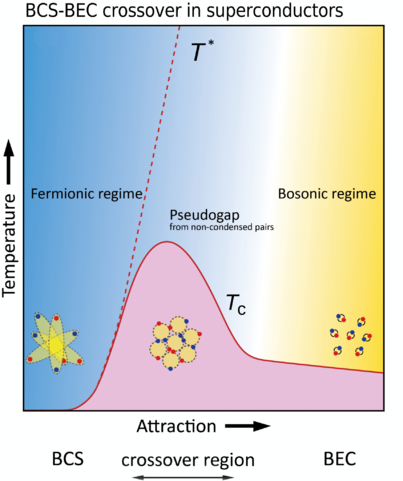
\includegraphics[width=0.46\textwidth]{images/BCS-BEC crossover.png}
	\caption[BCS-BEC crossover.]{
		\textbf{BCS-BEC crossover.} This is a general illustration of the crossover between loosely bound (BCS regime) and tightly bound (BEC regime) pairs in superconductors. 
		The crossover begins at the point where the pair creation temperature \(T^*\) diverges from the superconducting transition temperature \(T_{\mathrm{C}}\), at which the pairs condense.
		Reprinted figure with permission from \cite{chenWhenSuperconductivityCrosses2024}. Copyright 2024 by the American Physical Society.}
	\label{fig:BCS-BEC-crossover}
\end{SCfigure}
One topic emerging in the context of high-\(T_{\mathrm{C}}\) superconductors is the description in the BCS-BEC crossover \cite{chenWhenSuperconductivityCrosses2024}.
It is a framework independent of the specific pairing mechanism and characterizes superconductivity on the axis of weak to strong coupling.
\Cref{fig:BCS-BEC-crossover} shows the two regimes that can be connected by tuning the generalized coupling: the BCS regime with large electron pairs and the Bose-Einstein condensate regime with tightly bound pairs.
The \(T_{\mathrm{C}}\) in \cref{fig:BCS-BEC-crossover} has a dome-shape going from the weak to strong pairing, which is reminiscent of the dome shape against doping in many unconventional superconductors such as the Cuprates.

One indication that this description might have application for unconventional superconductors is given in the `Uemura' plot \cref{fig:Uemura plot} \cite{uemuraUniversalCorrelationsT_C1989, uemuraBasicSimilaritiesCuprate1991, uemuraCondensationExcitationPairing2004, uemuraDynamicSuperconductivityResponses2019a}.
Here, the critical temperature \(T_{\mathrm{C}}\) is compared to the available kinetic energy scale of superconducting charge carriers characterized by an effective Fermi temperature \(T_{\mathrm{F}}\).
Most unconventional superconductors show a linear scaling \(T_{\mathrm{C}} \propto T_{\mathrm{F}}\) across material families and fall into a limited region of \(\nicefrac{T_{\mathrm{C}}}{T_{\mathrm{F}}} \sim \numrange{0.01}{0.06}\).
This suggests that a BCS-BEC crossover description by a single parameter \(n_{\mathrm{s}}\) (or equivalently \(D_{\mathrm{S}} \propto \frac{n_{\mathrm{s}}}{m^*}\) with the effective mass of charge carriers \(m^*\)) might be applicable.

\begin{figure}[tb]
	\centering
	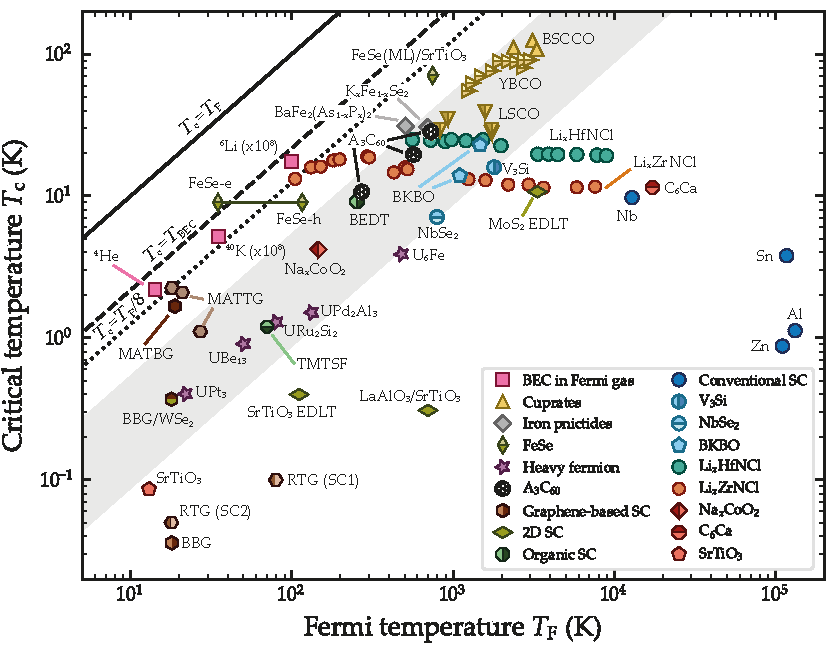
\includegraphics[width=0.8\textwidth]{images/Uemura_plot.pdf}
	\caption[Uemura plot.]{\textbf{Uemura plot.} 
		Comparison of Fermi temperature \(T_{\mathrm{F}}\) and critical temperature \(T_{\mathrm{C}}\) for various families of superconductors on a logarithmic plot.
		The gray shaded region marks the regime where most unconventional superconductors are located (here \(T_{\mathrm{C}} = 0.04 T_{\mathrm{BEC}}\) to \(T_{\mathrm{C}} = 0.25 T_{\mathrm{BEC}}\)).
		The lines mark different limits for \(T_{\mathrm{C}}\): the solid line being \(T_{\mathrm{C}} = T_{\mathrm{F}}\), the dashed line is the critical temperature of a non-interacting BEC (\(T_{\mathrm{BEC}} = \nicefrac{T_{\mathrm{F}}}{4.16}\)) and the upper limit for the Berezinski–Kosterlitz–Thouless transition of free electrons in two dimensions \(T_{\mathrm{C}} = \nicefrac{T_{\mathrm{F}}}{8}\) as a dotted line.
		Taken from \cite{wittElectronCorrelationsUnconventional} with data from \cite{nakagawaGatecontrolledBCSBECCrossover2021, uemuraDynamicSuperconductivityResponses2019, pantaleonSuperconductivityCorrelatedPhases2023a}.
	}
	\label{fig:Uemura plot}
\end{figure}

The intermediate region is characterized by the fact that despite the electron pairing strength being increased (marked by \(T^*\)), there is no superconductivity.
This is due to the fact that besides pairing, also phase coherence is needed for superconducting order which is suppressed as the stronger attraction impairs pair mobility.
The BCS-BEC crossover phenomenology gives qualitative insights in what limits \(T_{\mathrm{C}}\), which is again strongly connected to the superconducting length scales: in the BCS regime, the energy scale that limits \(T_{\mathrm{C}}\) is the pairing energy \(\Delta\) which is related to the coherence length \(\xi_0\) while in the BEC regime it is the phase coherence energy \(D_{\mathrm{S}}\) which is directly related to the London penetration depth \(\lambda_{\mathrm{L}, 0}\) via \(D_{\mathrm{S}} = \lambda_{\mathrm{L}, 0}^{-2}\).
This gives a possible route to raising \(T_{\mathrm{C}}\) by evading the constraints of the BCS-BEC crossover in the strong-coupling regime \cite{emeryImportancePhaseFluctuations1995, kivelsonMakingHighTc2002}.
This is explored for the example of Alkali-doped fullerides in ref. \cite{wittBypassingLatticeBCS2024}: by exploiting the high degrees of freedom in this multi-orbital system, the typical constraint on the superfluid stiffness imposed by the lattice can be evaded, enabling high \(T_{\mathrm{C}}\).

A similar avenue for evading constraints on \(T_{\mathrm{C}}\) is flat-band systems.
A flat electronic band corresponds to a large density of states at the Fermi level, which supports pairing in BCS theory.
On the other hand, the superfluid weight for a single band is its curvature, so zero in the flat-band case.
In multiband systems, the geometry of the space spanned by the electronic Bloch states (the so-called quantum geometry) gives a contribution that can be non-zero even for flat-band systems \cite{peottaSuperfluidityTopologicallyNontrivial2015, penttilaFlatbandRatioQuantum2025}.

\subsection*{Strong Correlations in Graphene Based Systems}

Graphene, the two-dimensional allotrope of Carbon was first synthesized in 2004 \cite{novoselovElectricFieldEffect2004}.
It sparked the field of 2D materials, which shows unique properties due to the confinement in one dimension and extensive tunability with environmental dielectric screening, electrostatic doping or tuning with external fields \cite{geimVanWaalsHeterostructures2013}.

Over time, another tuning parameter emerged: it turned out that two graphene layer twisted against each other as seen in \cref{sfig:3D printed twisted graphene} host localized electrons with pronounced interaction effects for certain twist angles.
In 2018, \citeauthor{caoUnconventionalSuperconductivityMagicangle2018} measured superconductivity in this setup with a phase diagram very similar to the Cuprates \cite{caoUnconventionalSuperconductivityMagicangle2018}.
Another method to enhance interaction effects in graphene based systems are multilayer systems without twisting, such as Bernal bilayer, ABC or ABCA layered systems \cite{pantaleonSuperconductivityCorrelatedPhases2023}.

For these systems, the strong quantum geometry comes from the graphene Dirac cones \cite{wehlingDiracMaterials2014}, playing a role in stabilizing superconducting \cite{peottaSuperfluidityTopologicallyNontrivial2015, liangBandGeometryBerry2017, tanakaSuperfluidStiffnessMagicangle2025, tianEvidenceDiracFlat2023, xieTopologyBoundedSuperfluidWeight2020, huGeometricConventionalContribution2019} and magnetic order \cite{abouelkomsanQuantumMetricInduced2023, liuOrbitalMagneticStates2021} in the multilayer systems.
\begin{figure}[tb]
	\begin{subfigure}[b]{0.5\textwidth}
		\centering
		\caption{\hfill\null}\label{sfig:3D printed twisted graphene}
		\includegraphics[width=0.75\textwidth]{images/Twisted 3D printed graphene small.png}
	\end{subfigure}%
	\begin{subfigure}[b]{0.5\textwidth}
		\centering
		\caption{\hfill\null}\label{sfig:unconventional SC MATBG}
		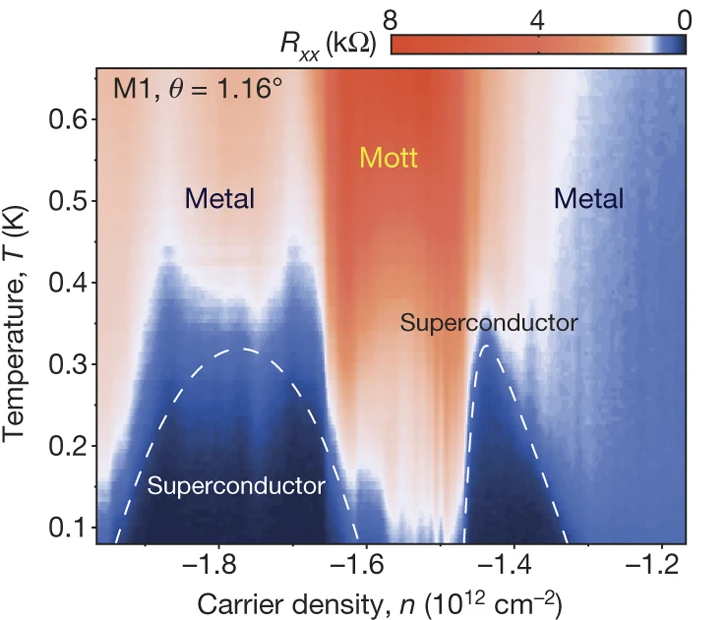
\includegraphics[width=1.0\textwidth]{images/cao_unvoncentional_SC_MATBG.png}
	\end{subfigure}%
	\caption[Twisted Bilayer graphene.]{
		\textbf{Twisted Bilayer graphene.} \textbf{(\subref{sfig:3D printed twisted graphene})} Moiré pattern formed by imposing two hexagonal lattices on top of each other with a twist angle. The emerging pattern has brighter regions where the layer approximately align and darker regions where the top-layer atoms in the \(\mathrm{A}\) sublattice sit roughly above the \(\mathrm{B}\) atoms in the bottom layer, but the top-layer \(\mathrm{B}\) atoms have no partner in the bottom layer.
		\textbf{(\subref{sfig:unconventional SC MATBG})} Phase diagram of the twisted bilayer graphene at a twist angle of \(\qty{1.16}{\degree}\) showing the dependence of \(T_{\mathrm{C}}\) on the carrier density in the partially filled flat band.
		Reproduced from \cite{caoUnconventionalSuperconductivityMagicangle2018} with permission from Springer Nature.
	}
\end{figure}
In the Uemura plot \cref{fig:Uemura plot}, twisted Bilayer and Trilayer graphene are very close to the theoretical 2D limit \cite{hazraBoundsSuperconductingTransition2019} and they lie outside the line of most unconventional superconductors.
This makes them very `efficient': they show a high \(T_{\mathrm{C}}\) for their low Fermi temperature/carrier density, so further efforts in the class of graphene-based flat-band systems might lead to key insights into superconductivity with even higher \(T_{\mathrm{C}}\).

\subsection*{Organization of this thesis}

The graphene structures discussed above are an interesting class for novel superconductors in itself and the insight gained from them informs many other avenues to better superconducting materials. 
In light of this, a conceptually simple model that captures relevant ingredients of the strong superconductivity in these systems is investigated in this thesis, namely a flat band and robust quantum geometry inherited from the graphene band structure.
The model is not only useful to better understand general aspects of superconductivity in other flat band graphene structures, but it can also be experimentally realized in adatom heterostructures \cite{ghosalElectronicCorrelationsEpitaxial2024, wittQuantumGeometryLocal2025}.
These have inherently larger energy scale on the order of the hopping in graphene (\(\mathcal{O} (\unit{\electronvolt})\)) in comparison to the inherent energy scales of Moiré and multilayer structures (\(\mathcal{O} (\unit{\milli\electronvolt})\)), which means that also correlated phenomena like the flat band superconductivity might persist to higher temperatures.

To fully characterize superconductivity in this model, the coherence length \(\xi_0\) and the London penetration depth \(\lambda_{\mathrm{L}, 0}\) are calculated.
This is done by analyzing the breakdown of the superconducting order parameter under the constraint of \gls{fmp}.

\Cref{ch:superconductivity} reviews aspects of the theoretical description of superconductors, in particular Ginzburg-Landau theory, whose framework is used to evaluate the \gls{fmp} ansatz.
Furthermore, \gls{bcs} theory and \gls{dmft} under the \gls{fmp} constraint are explained.
The decorated graphene model and its experimental basis are reviewed in \cref{ch:decorated graphene model}.
The \gls{fmp} method is then applied in \cref{ch:results}, in the \gls{bcs} formulation for the decorated graphene model and in the \gls{dmft} formulation for the simpler one band Hubbard model on the square lattice.
In the last chapter (\cref{ch:conclusion}), further pathways for investigation using the tools discussed in the thesis are presented.

\end{document}